
\begin{appendices}

\addtocontents{toc}{\protect\setcounter{tocdepth}{0}}

\chapter{Supplementary Material}

\section{Figures}

The contents...

\begin{figure}[ht]
	\begin{center}
\begin{tabular}{c}
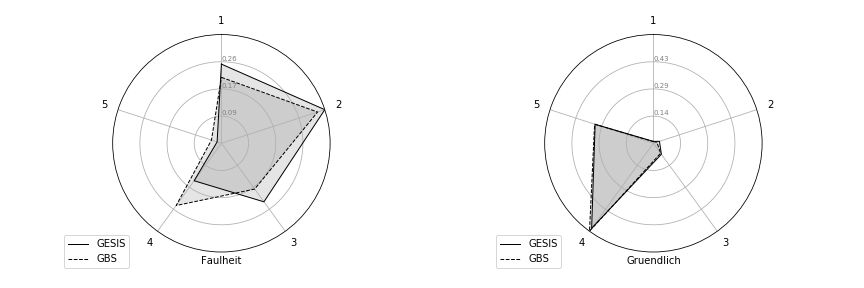
\includegraphics[scale=0.40,angle=0]{fig/Conscientiousness_figure} \\
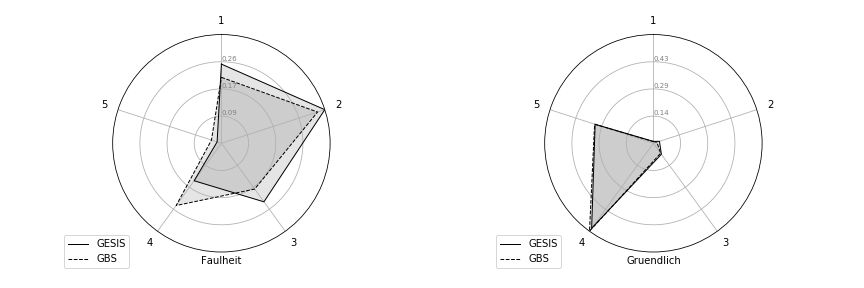
\includegraphics[scale=0.40,angle=0]{fig/Conscientiousness_figure} \\
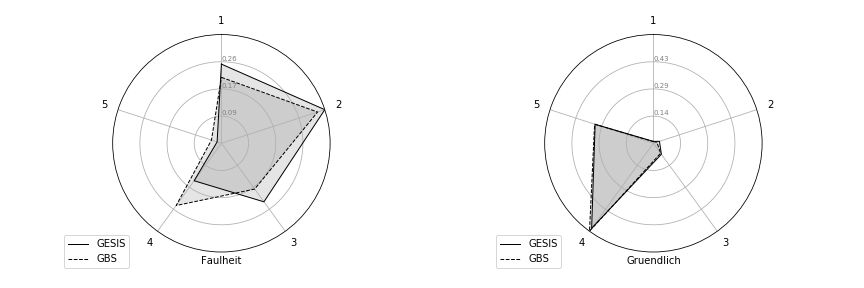
\includegraphics[scale=0.40,angle=0]{fig/Conscientiousness_figure} \\
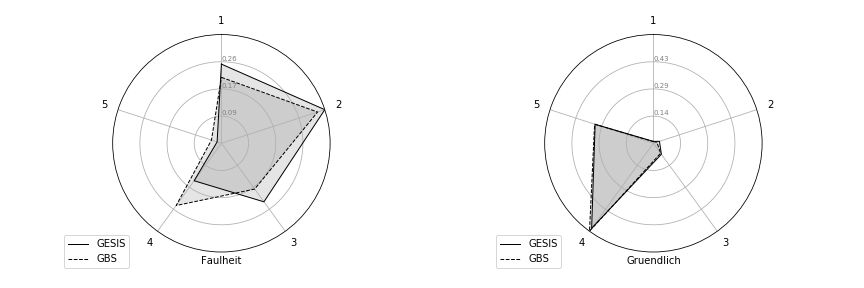
\includegraphics[scale=0.40,angle=0]{fig/Conscientiousness_figure} \\
\end{tabular}
\caption{caption}
\end{center}
\end{figure}

Agreeableness is the measure of one's cooperation, empathy, and willingness to trust and help others. Openness refers to openness to new experiences (i.e., whether one is timid/hesitant or eager about new objects or situations), level of inquisitiveness or curiousity, and level of preference for variety, novel stimuli and creativity. Extraversion refers to level of sociability, seeking and enjoyment of social contact, and energy and assertiveness in social situations. Extraverted people are outgoing and loquacious, while introverted people are reserved and favour solitude to social contact. Positive high affect (emotion) is linked to this concept. Neuroticism is characterized by easily experiencing disagreeable or negative emotions (anger, disappointment, frustration, etc.), and a poor coping response to those emotions

\begin{figure}[ht]
	\begin{center}
		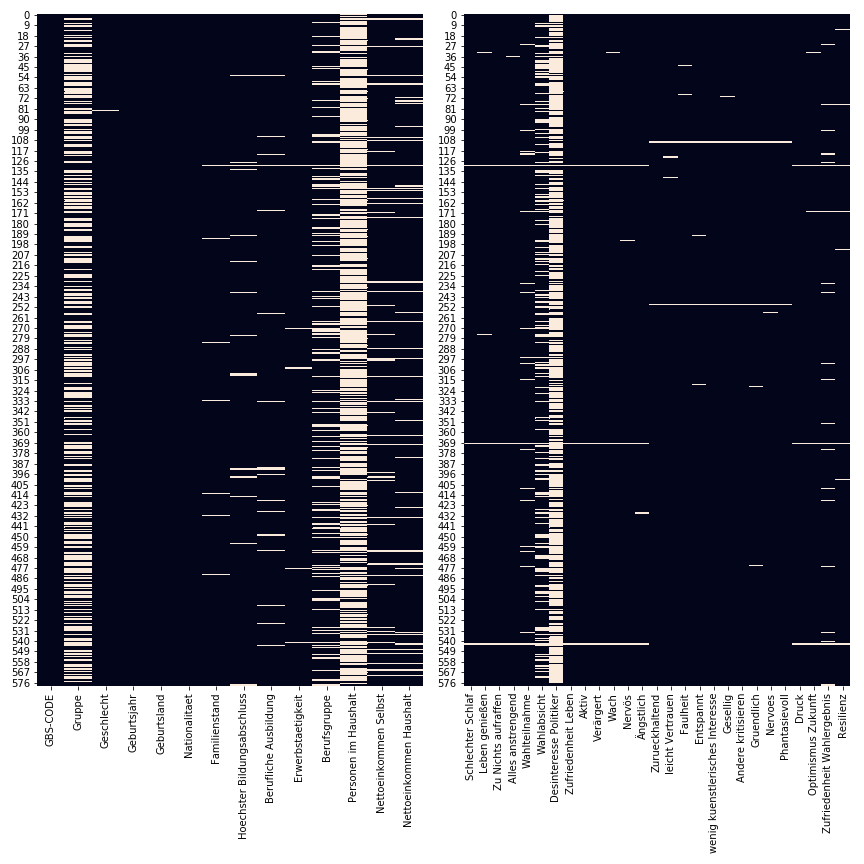
\includegraphics[scale=0.52,angle=0]{fig/gbs_missing}
		\label{std}
		\caption{GBS - GESIS attribute and value comparison.}
	\end{center}
\end{figure}


\section{Tables}

\section{Code}

\pythonexternal{fig/latex.py}

\chapter{GitHub Repository}

\begin{figure}[ht]
	\begin{center}
		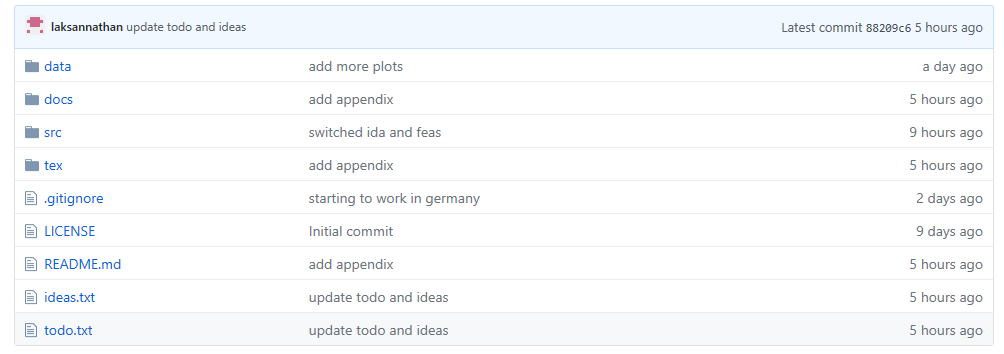
\includegraphics[scale=0.48,angle=0]{fig/github_a}
		\label{std}
	\end{center}
\end{figure}

\begin{figure}[ht]
	\begin{center}
		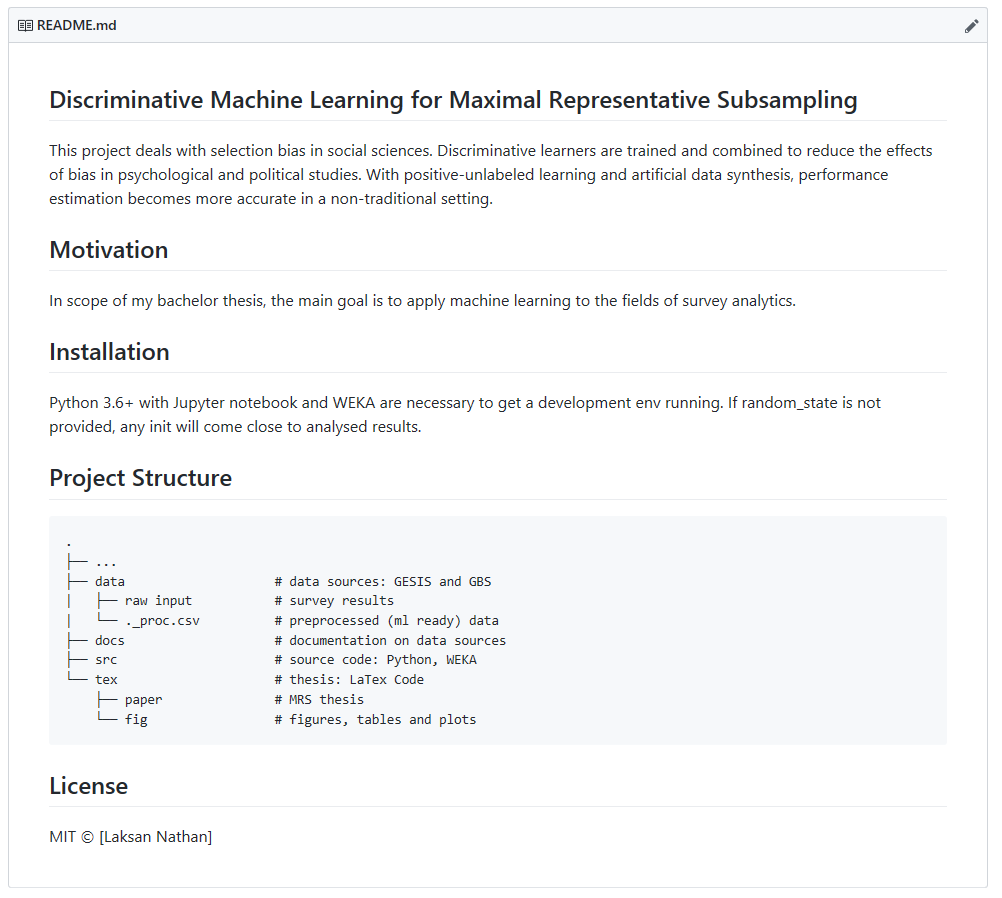
\includegraphics[scale=0.48,angle=0]{fig/github_b}
		\label{std}
	\end{center}
\end{figure}


\end{appendices}